\documentclass[
	a4paper,
	oneside,
	BCOR = 10mm,
	DIV = 12,
	12pt,
	headings = normal,
]{scrartcl}

%%% Length calculations
\usepackage{calc}
%%%

%%% Support for color
\usepackage{xcolor}
\definecolor{lightblue}{HTML}{03A9F4}
\definecolor{red}{HTML}{F44336}
%%%

%%% Including graphics
\usepackage{graphicx}
%%%

%%% Font selection
\usepackage{fontspec}

\setromanfont{STIX Two Text}[
	SmallCapsFeatures = {LetterSpace = 8},
]

\setsansfont{IBM Plex Sans}[
	Scale = MatchUppercase,
]

\setmonofont{IBM Plex Mono}[
	Scale = MatchUppercase,
]
%%%

%%% Math typesetting
\usepackage{amsmath}

\usepackage{unicode-math}
\setmathfont{STIX Two Math}

\usepackage{IEEEtrantools}
%%%

%%% List settings
\usepackage{enumitem}
\setlist[enumerate]{%
	label*      = {\arabic*.},
	left        = \parindent,
	topsep      = 0\baselineskip,
	parsep      = 0\baselineskip,
	itemsep     = 0\baselineskip,
	noitemsep, % override itemsep
}

\setlist[itemize]{%
	label       = {—},
	left        = \parindent,
	topsep      = 0\baselineskip,
	parsep      = 0\baselineskip,
	itemsep     = 0\baselineskip,
	noitemsep, % override itemsep
}

\setlist[description]{%
	font        = {\rmfamily\upshape\bfseries},
	topsep      = 1\baselineskip,
	parsep      = 0\baselineskip,
	itemsep     = 0\baselineskip,
}

%%%

%%% Structural elements typesetting
\setkomafont{pagenumber}{\rmfamily\upshape}
\setkomafont{disposition}{\rmfamily\bfseries}

% Sectioning
\RedeclareSectionCommand[
	beforeskip = -1\baselineskip,
	afterskip  = 1\baselineskip,
	font       = {\normalsize\bfseries\scshape},
]{section}

\RedeclareSectionCommand[
	beforeskip = -1\baselineskip,
	afterskip  = 1\baselineskip,
	font       = {\normalsize\bfseries\itshape},
]{subsection}

\RedeclareSectionCommand[
	beforeskip = -1\baselineskip,
	afterskip  = 1\baselineskip,
	font       = {\normalsize\bfseries},
]{subsubsection}

\RedeclareSectionCommand[
	beforeskip = -1\baselineskip,
	afterskip  = -0.5em,
	font       = {\normalsize\mdseries\scshape\addfontfeatures{Letters = {UppercaseSmallCaps}}},
]{paragraph}
%%%

%%% Typographic enhancements
\usepackage{microtype}
%%%

%%% Language-specific settings
\usepackage{polyglossia}
\setmainlanguage{ukrainian}
\setotherlanguages{english}
%%%

%%% Captions
\usepackage{caption}
\usepackage{subcaption}

%\DeclareCaptionLabelFormat{closing}{#2)}
%\captionsetup[subtable]{labelformat = closing}

%\captionsetup[subfigure]{labelformat = closing}

\captionsetup[table]{%
	aboveskip = 0\baselineskip,
	belowskip = 0\baselineskip,
}

\captionsetup[figure]{%
	aboveskip = 1\baselineskip,
	belowskip = 0\baselineskip,
}

\captionsetup[subfigure]{%
	labelformat = simple,
	labelformat = brace,
}
%%%

%%% Hyphenated ragged typesetting
\usepackage{ragged2e}
%%%

%%% Table typesetting
\usepackage{booktabs}
\usepackage{longtable}

\usepackage{multirow}

\usepackage{array}
\newcolumntype{v}[1]{>{\RaggedRight\arraybackslash\hspace{0pt}}p{#1}}
\newcolumntype{b}[1]{>{\Centering\arraybackslash\hspace{0pt}}p{#1}}
\newcolumntype{n}[1]{>{\RaggedLeft\arraybackslash\hspace{0pt}}p{#1}}
%%%

%%% Drawing
\usepackage{tikz}
\usepackage{tikzscale}
\usetikzlibrary{arrows.meta} % Stealth arrow tips
\usetikzlibrary{calc} % Coordinate calculations
\usetikzlibrary{positioning}
\usetikzlibrary{shapes.geometric} % Stealth arrow tips
%%%

%%% SI units typesetting
\usepackage{siunitx}
\sisetup{%
	output-decimal-marker = {,},
	exponent-product      = {\cdot},
	inter-unit-product    = \ensuremath{{} \cdot {}},
	per-mode              = symbol,
}
%%%

%%% Framing code listings
\usepackage{tcolorbox}
\tcbuselibrary{breakable}
\tcbuselibrary{minted}
\tcbuselibrary{skins}

\newtcblisting[
	auto counter,
	list inside,
	number within = section,
]{listingpython}[3][]{%
	minted language = python,
	minted style    = bw,
	minted options  = {%
		linenos,
		tabsize = 4,
		breaklines,
		% breakanywhere,
		fontsize = \footnotesize,
		autogobble
	},
	%
	% empty,
	sharp corners,
	colframe         = black,
	colback          = black!0,
	leftrule         = 0em,
	rightrule        = 0em,
	toprule          = 1pt, % orig = 0pt
	bottomrule       = 1pt, % orig = 0pt
	titlerule        = 0.5pt,
	colbacktitle     = black!0,
	coltitle         = black,
	toptitle         = 0.3em,
	bottomtitle      = 0.1em,
	borderline north = {1pt}{0pt}{black},
	borderline south = {1pt}{0pt}{black},
	before skip      = \intextsep,
	after  skip      = \intextsep,
	title            = {Лістинг \thetcbcounter: #2},
	list entry       = {\protect\numberline{\thetcbcounter}#2},
	left = 0em,
	right = 0em,
	%
	listing only,
	breakable,
	%
	label = {#3},
	%
	#1
}

\newtcbinputlisting[auto counter, list inside, number within = section]{\inputpython}[4][]{%
	minted language = python,
	minted style    = bw,
	minted options  = {%
		linenos,
		tabsize = 4,
		breaklines,
		breakbytokenanywhere,
		fontsize = \footnotesize,
	},
	%
	% empty,
	sharp corners,
	colframe         = black,
	colback          = black!0,
	leftrule         = 0em,
	rightrule        = 0em,
	toprule          = 0pt, % orig = 0pt
	bottomrule       = 0pt, % orig = 0pt
	titlerule        = 0.5pt,
	colbacktitle     = black!0,
	coltitle         = black,
	toptitle         = 0.3em,
	bottomtitle      = 0.1em,
	borderline north = {1pt}{0pt}{black},
	borderline south = {1pt}{0pt}{black},
	before skip      = \intextsep,
	after  skip      = \intextsep,
	title            = {Лістинг \thetcbcounter: #3},
	list entry       = {\protect\numberline{\thetcbcounter}#3},
	left = 0em,
	right = 0em,
	%
	listing file={#2},
	listing only,
	breakable,
	%
	label = {#4},
	%
	#1
}

% Customize minted
\usepackage{minted}
\setmintedinline{%
	style = bw,
	breaklines,
}

% Customize minted line numbers
\renewcommand{\theFancyVerbLine}{\ttfamily\scriptsize\arabic{FancyVerbLine}}

%%%

%%% Sideways floats
\usepackage{pdflscape}
\usepackage{afterpage} % wrap landscape floats
%%%

%%% Wrap text after sideways table
\usepackage{afterpage}
%%%

%%% Links and hyperreferences
\usepackage{hyperref}
\hypersetup{%
	bookmarksnumbered = true,
	colorlinks      = false,
	linkbordercolor = red,
	urlbordercolor  = lightblue,
	pdfborderstyle  = {/S/U/W 1.5},
}
%%%

%%% Length adjustments
% Set baselineskip, default is 14.5 pt
\linespread{1.068966} % ~15.5 pt
\setlength{\emergencystretch}{1em}
\setlength{\parindent}{1.5em}
\newlength{\gridunitwidth}
\setlength{\gridunitwidth}{\textwidth / 12}
%%%

%%% Custom commands
\newcommand{\allcaps}[1]{{\addfontfeatures{LetterSpace = 8, Kerning = Off}#1}}
\newcommand{\filename}[1]{\texttt{#1}}
\newcommand{\progname}[1]{\texttt{#1}}
\newcommand{\modulename}[1]{\texttt{#1}}
%%%

%%% Custom math commands
\newcommand{\longvar}[1]{\mathit{#1}}
\newcommand{\sdiv}{\mathbin{/}}
%%%

\begin{document}

\begin{titlepage}
		\begin{center}
			Міністерство освіти і~науки України\\
			Національний авіаційний університет\\
			Навчально-науковий інститут комп'\-ютерних інформаційних технологій\\
			Кафедра комп'\-ютеризованих систем управління

			\vspace{\fill}
				Лабораторна робота №6\\
				з~дисципліни «Комп'\-ютерні системи»\\
				на~тему «Аналіз функціонування конвеєрних обчислювальних систем»\\
				Варіант~№3

			\vspace{\fill}

			\begin{flushright}
				Виконав:\\
				студент \allcaps{ННІКІТ}\\
				групи СП-325\\
				Клокун В.\,Д.\\
				Перевірив:\\
				Ковальов М.\,О.
			\end{flushright}

			Київ 2019
		\end{center}
	\end{titlepage}

	\section{Мета роботи}
		Аналіз функціонування та~ефективності конвеєрних обчислювальних систем.

	\section{Загальні теоретичні відомості}
		Критерії ефективності конвеєрної системи. Які критерії ефективності розв’язання задачі (обчислення арифметичних виразів) будемо розглядати:
		\begin{enumerate}
			\item Коефіцієнт прискорення:
				\begin{IEEEeqnarray}{rCl}
					K_{\text{П}}
					= \frac{
						T_{0}
					}{
						T_{N}
					},
				\end{IEEEeqnarray}
				де~$T_0$~— час розв’язання задачі в~традиційній ЕОМ (однопроцесорній), який дорівнює сумі часів виконання операцій додавання, множення та~ділення; $T_{N}$~— час розв’язання задачі в~конвеєрній системі.
			\item Коефіцієнт завантаження конвеєра:
				\begin{IEEEeqnarray}{rCl}
					K_{\text{З}}
					= \frac{
						T_{0}
					}{
						N \cdot T_{N}
					},
				\end{IEEEeqnarray}
				де~$N$~— кількість шарів в~конвеєрі.
		\end{enumerate}

		\textit{Приклад.} Зробимо аналіз функціонування конвеєрних ОС~різних типів для заданого арифметичного виразу:
		\begin{IEEEeqnarray}{rCl}
			\label{eq:theory}
			(A + B) + C \sdiv D + G + (K \sdiv L + M + N).
		\end{IEEEeqnarray}

		Будь-який арифметичний вираз із~змінними можна графічно подати у~вигляді дерева. На~рис.~\ref{fig:theory-01} зображено дерево арифметичного виразу~\eqref{eq:theory}:
		\begin{figure}[!htbp]
			\centering
			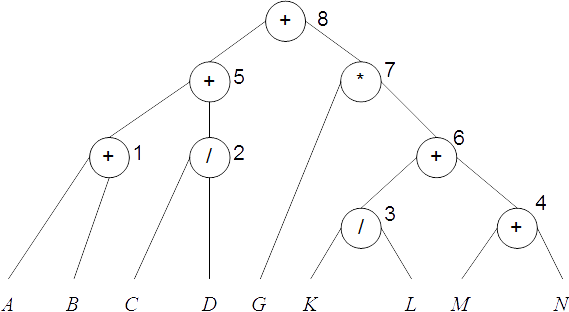
\includegraphics[height = 10\baselineskip]{./assets/y03s02-compsys-lab-06-p01.png}
			\caption{}
			\label{fig:theory-01}
		\end{figure}

		Час обчислення даного арифметичного виразу в~традиційній ЕОМ можна визначити таким чином:
		\begin{IEEEeqnarray}{rCl}
			T_{0} = 5 T_{\text{с}} + 2 T_{\text{д}} + T_{\text{м}} ,
		\end{IEEEeqnarray}
	де~$T_{\text{с}}$~— час операції додавання, $T_{\text{с}}$~— час операції ділення, $T_{\text{с}}$~— час операції множення.

		Нехай задано $τ_{\text{с}} = 1$, $τ_{\text{м}} = 2 τ_{\text{с}}$, $τ_{\text{с}} = 5 τ_{\text{с}}$, де~$τ_{\text{с}}$~— час операції додавання в~одному шарі конвеєра, $\tau_{\text{д}}$ – час операції ділення в~одному шарі конвеєра, $\tau_{\text{д}}$~— час операції множення в~одному шарі конвеєра. Відповідно $T_{\text{с}} = N \cdot \tau_{\text{с}}$; $T_{\text{д}}= N \cdot 5 \cdot \tau_{\text{с}}$; $Т_{\text{м}} = N \cdot 2 \cdot \tau_{\text{с}}$. Тоді при послідовному виконанні всіх операцій даного виразу в~конвеєрі з~$N=4$, де~$N$ – кількість шарів конвеєра $T_{0}=5 \cdot 4 \cdot τ_{\text{с}} +2 \cdot 4 \cdot 5 \cdot τ_{\text{с}} + 4 \cdot 2 \cdot τ_{\text{с}} =68 τ_{\text{с}}$. 

		\begin{enumerate}
			\item Розглянемо діаграму роботи конвеєра з~динамічною перебудовою, наведеного на~рис.~\ref{fig:theory-01}, для випадку з~$N=4$ (рис.~\ref{fig:theory-02}).

			\begin{figure}[!htbp]
				\centering
				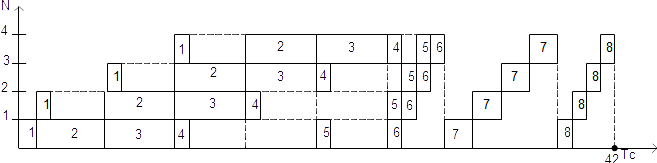
\includegraphics[width = \columnwidth]{./assets/y03s02-compsys-lab-06-p02.png}
				\caption{Діаграма роботи конвеєра з~динамічною перебудовою}
				\label{fig:theory-02}
			\end{figure}

			Використовуючи вирази (1) та~(2), визначимо коефіцієнти прискорення та~завантаження:
			\begin{IEEEeqnarray*}{rCl}
				K_{\text{п}} = \frac{T_{0}}{T_{\text{дин}}} = \num{1.62}, \quad
				K_{\text{з}} = \frac{T_{0}}{N \cdot T_{\text{дин}}} = \num{0.405}.
			\end{IEEEeqnarray*}

		\item Розглянемо діаграму роботи конвеєра зі~статичною перебудовою (рис. 3).

			\begin{figure}[!htbp]
				\centering
				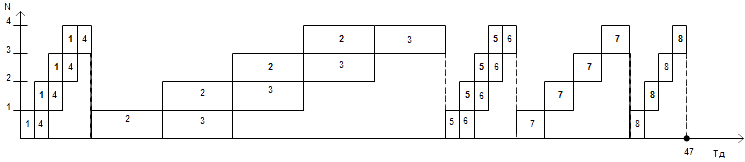
\includegraphics[width = \columnwidth]{./assets/y03s02-compsys-lab-06-p03.png}
				\caption{Діаграма роботи конвеєра зі~статичною перебудовою}
				\label{fig:theory-03}
			\end{figure}

			Використовуючи вирази (1) та~(2), визначимо коефіцієнти прискорення та~завантаження:
			\begin{IEEEeqnarray*}{rCl}
				K_{\text{п}} = \frac{T_{0}}{T_{\text{дин}}} = \num{1.45}, \quad
				K_{\text{з}} = \frac{T_{0}}{N \cdot T_{\text{дин}}} = \num{0.362}.
			\end{IEEEeqnarray*}
		\item Розглянемо діаграму роботи конвеєра з~постійним тактом (рис. 4).
		\begin{figure}[!htbp]
			\centering
			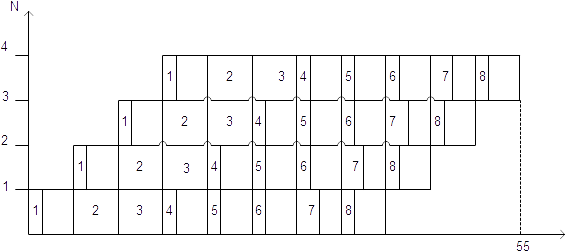
\includegraphics[height = 8\baselineskip]{./assets/y03s02-compsys-lab-06-p04.png}
			\caption{Діаграма роботи конвеєра з~постійним тактом}
			\label{fig:theory-04}
		\end{figure}
		Використовуючи вирази (1) та~(2), визначимо коефіцієнти прискорення та~завантаження:
			\begin{IEEEeqnarray*}{rCl}
				K_{\text{п}} = \frac{T_{0}}{T_{\text{дин}}} = \num{1.24}, \quad
				K_{\text{з}} = \frac{T_{0}}{N \cdot T_{\text{дин}}} = \num{0.309}.
			\end{IEEEeqnarray*}
		\end{enumerate}

		В~табл. 1 наведено значення коефіцієнтів прискорення та~завантаження під час розв’язання задачі обчислення арифметичного виразу в~конвеєрах різних типів.
			\begin{table}[!htbp]
				\centering
				\caption{Значення коефіцієнтів прискорення та~завантаження}
				\label{tab:theory-01}
				\begin{tabular}{
					v{8\gridunitwidth - 2\tabcolsep}
					n{2\gridunitwidth - 2\tabcolsep}
					n{2\gridunitwidth - 2\tabcolsep}
				}
					\toprule
						Тип конвеєра & 
						$K_{\text{п}}$ &
						$K_{\text{з}}$ \\
					\midrule
						З~динамічною перебудовою К2.1 &
						\num{1,62} &
						\num{0,405} \\
						Зі~статичною перебудовою К2.2 &
						\num{1,45} &
						\num{0,362} \\
						З~постійним тактом К1 &
						\num{1,24} &
						\num{0,309} \\
					\bottomrule
				\end{tabular}
			\end{table}

		Аналіз результатів ефективності конвеєрів різних типів під час розв’язання задачі, що~розглядається, дозволяє зробити такі висновки:
		\begin{itemize}
			\item використання конвеєру типу К2.1 дозволяє розв’язати задачу за~мінімальний час;
			\item за~ступенем використання обладнання (завантаження конвеєра) перевагу слід віддати конвеєру типу К2.1. 
		\end{itemize}

	\section{Хід роботи}
		Вихідними даними для виконання лабораторної роботи за~варіантом №~8 є~арифметичний вираз~\eqref{eq:expr}:
		\begin{IEEEeqnarray}{rCl}
			\label{eq:expr}
			(A + B \sdiv C \times G) \times (K + E + L) \sdiv R + D.
		\end{IEEEeqnarray}
		За~даним виразом складаємо його дерево~— граф потоків обчислень~(рис.~\ref{fig:expression-tree}).

		\begin{figure}[!htbp]
			\centering
			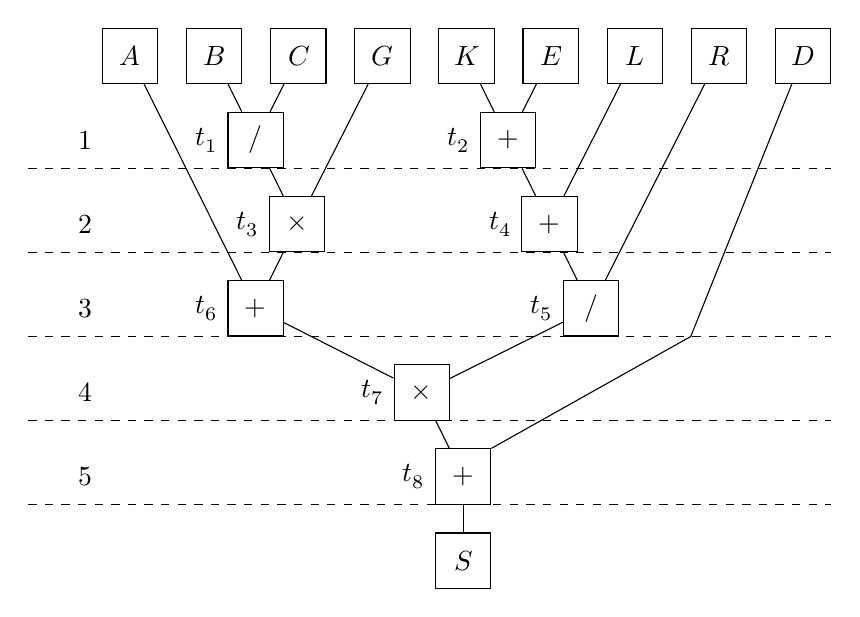
\begin{tikzpicture}[]
				\tikzset{main node/.style={draw,minimum size=2em}}
				\tikzset{every label/.style={label position=left}}
				\begin{scope}
					\node[main node] (l05-a) {$A$};
					\node[main node, right = 1em of l05-a] (l05-b) {$B$};
					\node[main node, right = 1em of l05-b] (l05-c) {$C$};
					\node[main node, right = 1em of l05-c] (l05-g) {$G$};
					\node[main node, right = 1em of l05-g] (l05-k) {$K$};
					\node[main node, right = 1em of l05-k] (l05-e) {$E$};
					\node[main node, right = 1em of l05-e] (l05-l) {$L$};
					\node[main node, right = 1em of l05-l] (l05-r) {$R$};
					\node[main node, right = 1em of l05-r] (l05-d) {$D$};
				\end{scope}

				\begin{scope}[every node/.style = {anchor=north west}]
					% Level 01
					\node[main node, label={$t_1$}, below right = 1em and 1.50em of l05-b.south west]  (l04-div-01) {$\sdiv$};
					\node[main node, label={$t_2$}, below right = 1em and 1.50em of l05-k.south west]  (l04-add-01) {$+$};

					% Level 02
					\node[main node, label={$t_3$}, below right = 1em and 1.50em of l04-div-01.south west]  (l03-mul-01) {$\times$};
					\node[main node, label={$t_4$}, below right = 1em and 1.50em of l04-add-01.south west]  (l03-add-01) {$+$};

					% Level 03
					\node[main node, label={$t_6$}, below left  = 1em and 1.50em of l03-mul-01.south east] (l02-add-01) {$+$};
					\node[main node, label={$t_5$}, below right = 1em and 1.50em of l03-add-01.south west] (l02-div-01) {$\sdiv$};

					% Level 04
					\node[main node, label={$t_7$}, below right = 1em and 6.00em of l02-add-01.south west] (l01-mul-01) {$\times$};

					% Level 05
					\node[main node, label={$t_8$}, below right = 1em and 1.50em of l01-mul-01.south west] (root-plus) {$+$};

					% Root
					\node[main node, below = 1em of root-plus] (root-S) {$S$};
				\end{scope}

				\begin{scope}
					\path[draw]
					(root-S)     edge node {} (root-plus)
					% Make intermediate point at horizontal intersection of t_5 and D
					(root-plus.north east)  -- (l02-div-01.south -| l05-r.south west) -- (l05-d)
					(root-plus)  edge node {} (l01-mul-01)
					(l01-mul-01) edge node {} (l02-add-01)
					             edge node {} (l02-div-01)
					(l02-add-01) edge node {} (l05-a)
					             edge node {} (l03-mul-01)
					(l02-div-01) edge node {} (l03-add-01)
					             edge node {} (l05-r)
					(l03-mul-01) edge node {} (l04-div-01)
					             edge node {} (l05-g)
					(l03-add-01) edge node {} (l04-add-01)
					             edge node {} (l05-l)
					(l04-div-01) edge node {} (l05-b)
					             edge node {} (l05-c)
					(l04-add-01) edge node {} (l05-k)
					             edge node {} (l05-e)
					;
				\end{scope}

				\begin{scope}
				%\path[dashed] (current bounding box.west) -- (current bounding box.east);
						\node [minimum size = 2em, anchor = north east, below left = 1em and 0em of l05-a.south west] (l05) {Ярус 1};
						\node [minimum size = 2em, below = 1em of l05.south] (l04) {Ярус 2};
						\node [minimum size = 2em, below = 1em of l04.south] (l03) {Ярус 3};
						\node [minimum size = 2em, below = 1em of l03.south] (l02) {Ярус 4};
						\node [minimum size = 2em, below = 1em of l02.south] (l01) {Ярус 5};

						\draw [dashed] (l05.south west) -- (l05.south west -| l05-d.east);
						\draw [dashed] (l04.south west) -- (l04.south west -| l05-d.east);
						\draw [dashed] (l03.south west) -- (l03.south west -| l05-d.east);
						\draw [dashed] (l02.south west) -- (l02.south west -| l05-d.east);
						\draw [dashed] (l01.south west) -- (l01.south west -| l05-d.east);
				\end{scope}

			\end{tikzpicture}
			\caption{Дерево арифметичного виразу $(A + B \sdiv C \times G) \times (K + E + L) \sdiv R + D$}
			\label{fig:expression-tree}
		\end{figure}
		Також дана кількість шарів у~конвеєрі~$N = 3$, значення коефіцієнта швидкості виконання множення~$\tau_{\times} = \tau_{\times} \sdiv \tau_{+} = 2$  і~коефіцієнта швидкості виконання ділення~$\tau_{\sdiv} = \tau_{\sdiv} \sdiv \tau_{+} = 4$.

		Оскільки у~виразі~\eqref{eq:expr} виконується 4~операції додавання, 2~операції множення і~2~операції ділення, то~час обчислення на~послідовній ЕОМ~$T_{0}$ такий:
		\begin{IEEEeqnarray*}{rCl}
			T_{0} = 4 T_{+} + 2 T_{\times} + 2 T_{\sdiv}.
		\end{IEEEeqnarray*}
		Визначимо тривалості виконання додавання~$T_{+}$, множення~$T_{\times}$ і~ділення~$T_{\sdiv}$ відповідно:
		\begin{IEEEeqnarray*}{rCl}
			T_{+}      &=& N \cdot \tau_{+}
			               = 3 \tau_{+},\\
			T_{\times} &=& N \cdot \tau_{\times} \cdot \tau_{+}
			               = 3 \cdot 2 \tau_{+} = 6 \tau_{+},\\
			T_{\sdiv}  &=& N \cdot \tau_{\sdiv} \cdot \tau_{+}
										 = 3 \cdot 4 \tau_{+} = 12 \tau_{+}.
		\end{IEEEeqnarray*}
		Отже, час обчислення на~послідовній ЕОМ~$T_{0}$ обчислюється так:
		\begin{IEEEeqnarray*}{rCl}
			T_{0} &=& 4 T_{+} + 2 T_{\times} + 2 T_{\sdiv}
						 = 4 \cdot 3\tau_{+} + 2 \cdot 6 \tau_{+} + 2 \cdot 12 \tau_{+}
						 = 12 \tau_{+} + 12 \tau_{+} + 24 \tau_{+}
						 = 48 \tau_{+}.
		\end{IEEEeqnarray*}
		Переходимо до~оцінки конвеєрних систем.

			\subsection{Конвеєр з~динамічною перебудовою (тип~К2.1)}
				Конвеєр з~динамічною перебудовою~(типу~K2.1) дозволяє виконувати різні операції в~одному такті. Однак, тривалість такту залежить від тривалості найбільш тривалої операції у~поточному такті. Складаємо часову діаграму~(рис.~\ref{fig:time-diag-pipeline-usage-k2p1}).

				\begin{figure}[!htbp]
					\centering
					\small
					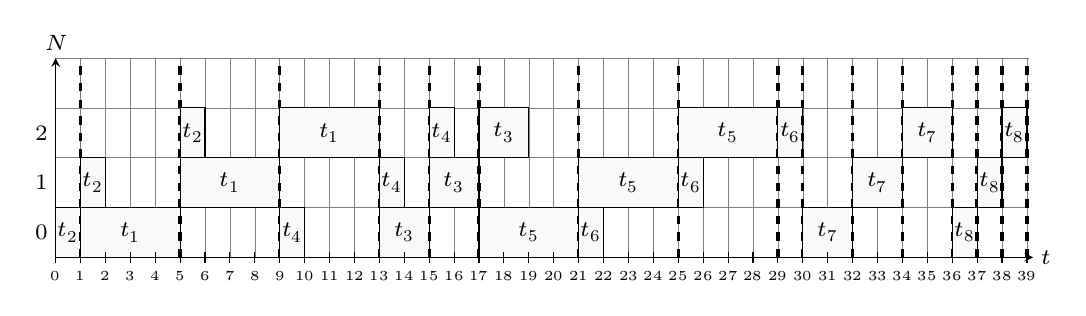
\begin{tikzpicture}[x = 0.9em, y = 1.8em]
						\footnotesize
						\draw[help lines, step=1] (0.0, 0.0) grid (39.1, 4.0);

						% Coordinate lines
						\begin{scope}[>=stealth]
							\draw[->] (0, 0) -- (39.25, 0) node[right] {$t$};
							\draw[->] (0, 0) -- (0, 4)   node[above] {$N$};
						\end{scope}

						\begin{scope}
							% step 1
							%
							\draw [fill = black!2.5]  (00,00) rectangle node {$t_2$} (01,01);
							\draw [dashed, very thick] (01,00) -- (01,04);
							% step 02
							%
							\draw [fill = black!2.5]  (01,00) rectangle node {$t_1$} (05,01);
							\draw [fill = black!2.5]  (01,01) rectangle node {$t_2$} (02,02);
							\draw [dashed, very thick] (05,00) -- (05,04);
							% step 03
							%
							\draw [fill = black!2.5]  (05,01) rectangle node {$t_1$} (09,02);
							\draw [fill = black!2.5]  (05,02) rectangle node {$t_2$} (06,03);
							\draw [dashed, very thick] (09,00) -- (09,04);
							% step 04
							\draw [fill = black!2.5] (09,00) rectangle node {$t_4$} (10,01);
							%\draw [fill = black!2.5] (05,01) rectangle node {$t_1$} (09,02);
							\draw [fill = black!2.5] (09,02) rectangle node {$t_1$} (13,03);
							\draw [dashed, very thick] (13,00) -- (13,04);
							% step 05
							\draw [fill = black!2.5]  (13,00) rectangle node {$t_3$} (15,01);
							\draw [fill = black!2.5]  (13,01) rectangle node {$t_4$} (14,02);
							\draw [dashed, very thick] (15,00) -- (15,04);
							%\draw [fill = black!2.5] (13,02) rectangle node {$t_2$} (13,03);
							% step 06
							%\draw [fill = black!2.5] (15,00) rectangle node {$t_3$} (15,01);
							\draw [fill = black!2.5]  (15,01) rectangle node {$t_3$} (17,02);
							\draw [fill = black!2.5]  (15,02) rectangle node {$t_4$} (16,03);
							\draw [dashed, very thick] (17,00) -- (17,04);
							% step 07
							\draw [fill = black!2.5]  (17,00) rectangle node {$t_5$} (21,01);
							% \draw [fill = black!2.5]  (17,01) rectangle node {$t_3$} (17,02);
							\draw [fill = black!2.5]  (17,02) rectangle node {$t_3$} (19,03);
							\draw [dashed, very thick] (21,00) -- (21,04);
							% step 08
							\draw [fill = black!2.5]  (21,00) rectangle node {$t_6$} (22,01);
							\draw [fill = black!2.5]  (21,01) rectangle node {$t_5$} (25,02);
							% \draw [fill = black!2.5]  (21,02) rectangle node {$t_3$} (19,03);
							\draw [dashed, very thick] (25,00) -- (25,04);
							% step 09
							% \draw [fill = black!2.5]  (25,00) rectangle node {$t_6$} (22,01);
							\draw [fill = black!2.5]  (25,01) rectangle node {$t_6$} (26,02);
							\draw [fill = black!2.5]  (25,02) rectangle node {$t_5$} (29,03);
							\draw [dashed, very thick] (29,00) -- (29,04);
							% step 10
							% \draw [fill = black!2.5]  (29,00) rectangle node {$t_6$} (22,01);
							% \draw [fill = black!2.5]  (29,01) rectangle node {$t_6$} (26,02);
							\draw [fill = black!2.5]  (29,02) rectangle node {$t_6$} (30,03);
							\draw [dashed, very thick] (30,00) -- (30,04);
							% step 11
							\draw [fill = black!2.5]  (30,00) rectangle node {$t_7$} (32,01);
							% \draw [fill = black!2.5]  (30,01) rectangle node {$t_6$} (26,02);
							% \draw [fill = black!2.5]  (30,02) rectangle node {$t_6$} (30,03);
							\draw [dashed, very thick] (32,00) -- (32,04);
							% step 12
							% \draw [fill = black!2.5]  (32,01) rectangle node {$t_6$} (26,02);
							\draw [fill = black!2.5]  (32,01) rectangle node {$t_7$} (34,02);
							% \draw [fill = black!2.5]  (32,02) rectangle node {$t_6$} (30,03);
							\draw [dashed, very thick] (34,00) -- (34,04);
							% step 13
							% \draw [fill = black!2.5]  (32,01) rectangle node {$t_6$} (26,02);
							% \draw [fill = black!2.5]  (32,00) rectangle node {$t_7$} (34,02);
							\draw [fill = black!2.5]  (34,02) rectangle node {$t_7$} (36,03);
							\draw [dashed, very thick] (36,00) -- (36,04);
							% step 14
							\draw [fill = black!2.5]  (36,00) rectangle node {$t_8$} (37,01);
							\draw [dashed, very thick] (37,00) -- (37,04);
							% step 15
							\draw [fill = black!2.5]  (37,01) rectangle node {$t_8$} (38,02);
							\draw [dashed, very thick] (38,00) -- (38,04);
							% step 16
							\draw [fill = black!2.5]  (38,02) rectangle node {$t_8$} (39,03);
							\draw [dashed, very thick] (39,00) -- (39,04);
						\end{scope}

						\newcommand*{\TickSize}{0.25em}
						% x ticks
						\begin{scope}
							\foreach \x in {0,...,39} {%
									\draw ($(\x,0) + (0,-\TickSize)$) -- ($(\x,0) + (0,\TickSize)$)
											node [anchor = north, below = 0.5em, font={\tiny}] {$\x$};
							}
						\end{scope}
						% y ticks
						% \begin{scope}
						% 	\foreach \y in {0,...,3} {%
						% 			\draw ($(0,\y) + (-\TickSize,0)$) -- ($(0,\y) + (\TickSize,0)$)
						% 					node [anchor = east, left = 1em] {CPU $\y$};
						% 	}
						% \end{scope}

						\begin{scope}
							\foreach \y in {0,...,2} {%
								\node[anchor = east] at (0, \y + 0.5) {$\y$};
							}
						\end{scope}
					\end{tikzpicture}
					\caption{Часова діаграма роботи конвеєра типу~K2.1 при~кількості шарів~$N = 3$}
					\label{fig:time-diag-pipeline-usage-k2p1}
				\end{figure}

				Як~видно на~осі~$Ot$, найдовший відрізок займає~39 одиниць, тобто виконання обчислення займає~$T_{K2.1} = 39t_{+}$.

				Обчисливши тривалість виконання обчислення на~обчислювальній системі типу K2.1 з~кількістю шарів~$N = 3$, обчислюємо її~критерії ефективності: коефіцієнт прискорення~$K_{\text{П}}$ і~коефіцієнт завантаження~$K_{\text{З}}$. Вони обчислюються так:
				\begin{IEEEeqnarray*}{rCl}
					K_{\text{П}} = \frac{T_0}{T_{K2.1}} = \frac{48 t_{+}}{39 t_{+}} = \num{1.231}, \quad
					K_{\text{З}} = \frac{T_0}{N \cdot T_{K2.1}} = \frac{48 t_{+}}{3 \cdot 39 t_{+}} = \num{0.410}.
				\end{IEEEeqnarray*}
				Отже, отримали характеристики ефективності конвеєрної системи типу~K2.1.

			\subsection{Конвеєр зі~статичною перебудовою (тип~К2.2)}
				Конвеєр зі~статичною перебудовою~(типу~K2.2) дозволяє виконувати в~одному такті операції одного типу, тому тривалість такту залежить від тривалості типу операцій у~поточному такті. Складаємо часову діаграму~(рис.~\ref{fig:time-diag-pipeline-usage-k2p2}).

				\begin{figure}[!htbp]
					\centering
					\small
					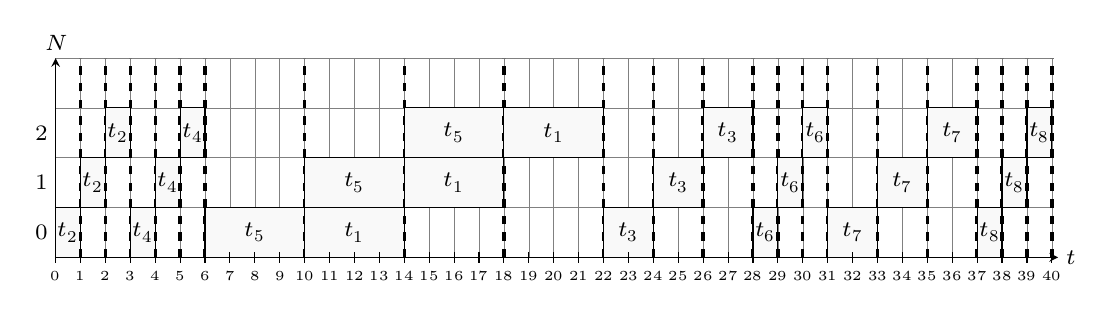
\begin{tikzpicture}[x = 0.9em, y = 1.8em]
						\footnotesize
						\draw[help lines, step=1] (0.0, 0.0) grid (40.1, 4.0);

						% Coordinate lines
						\begin{scope}[>=stealth]
							\draw[->] (0, 0) -- (40.25, 0) node[right] {$t$};
							\draw[->] (0, 0) -- (0, 4)   node[above] {$N$};
						\end{scope}

						\begin{scope}
							% step 01
							%
							\draw [fill = black!2.5]  (00,00) rectangle node {$t_2$} (01,01);
							\draw [dashed, very thick] (01,00) -- (01,04);
							% step 02
							%
							\draw [fill = black!2.5]  (01,01) rectangle node {$t_2$} (02,02);
							\draw [dashed, very thick] (02,00) -- (02,04);
							% step 03
							%
							\draw [fill = black!2.5]  (02,02) rectangle node {$t_2$} (03,03);
							\draw [dashed, very thick] (03,00) -- (03,04);
							% step 04
							%
							\draw [fill = black!2.5]  (03,00) rectangle node {$t_4$} (04,01);
							\draw [dashed, very thick] (04,00) -- (04,04);
							% step 05
							%
							\draw [fill = black!2.5]  (04,01) rectangle node {$t_4$} (05,02);
							\draw [dashed, very thick] (05,00) -- (05,04);
							% step 06
							%
							\draw [fill = black!2.5]  (05,02) rectangle node {$t_4$} (06,03);
							\draw [dashed, very thick] (06,00) -- (06,04);
							% step 07
							%
							\draw [fill = black!2.5]  (06,00) rectangle node {$t_5$} (10,01);
							\draw [dashed, very thick] (10,00) -- (10,04);
							% step 08
							%
							\draw [fill = black!2.5]  (10,00) rectangle node {$t_1$} (14,01);
							\draw [fill = black!2.5]  (10,01) rectangle node {$t_5$} (14,02);
							\draw [dashed, very thick] (14,00) -- (14,04);
							% step 09
							%
							\draw [fill = black!2.5]  (14,01) rectangle node {$t_1$} (18,02);
							\draw [fill = black!2.5]  (14,02) rectangle node {$t_5$} (18,03);
							\draw [dashed, very thick] (18,00) -- (18,04);
							% step 10
							%
							\draw [fill = black!2.5]  (18,02) rectangle node {$t_1$} (22,03);
							\draw [dashed, very thick] (22,00) -- (22,04);
							% step 11
							%
							\draw [fill = black!2.5]  (22,00) rectangle node {$t_3$} (24,01);
							\draw [dashed, very thick] (24,00) -- (24,04);
							% step 12
							%
							\draw [fill = black!2.5]  (24,01) rectangle node {$t_3$} (26,02);
							\draw [dashed, very thick] (26,00) -- (26,04);
							% step 13
							%
							\draw [fill = black!2.5]  (26,02) rectangle node {$t_3$} (28,03);
							\draw [dashed, very thick] (28,00) -- (28,04);
							% step 14
							%
							\draw [fill = black!2.5]  (28,00) rectangle node {$t_6$} (29,01);
							\draw [dashed, very thick] (29,00) -- (29,04);
							% step 15
							%
							\draw [fill = black!2.5]  (29,01) rectangle node {$t_6$} (30,02);
							\draw [dashed, very thick] (30,00) -- (30,04);
							% step 16
							%
							\draw [fill = black!2.5]  (30,02) rectangle node {$t_6$} (31,03);
							\draw [dashed, very thick] (31,00) -- (31,04);
							% step 17
							%
							\draw [fill = black!2.5]  (31,00) rectangle node {$t_7$} (33,01);
							\draw [dashed, very thick] (33,00) -- (33,04);
							% step 18
							%
							\draw [fill = black!2.5]  (33,01) rectangle node {$t_7$} (35,02);
							\draw [dashed, very thick] (35,00) -- (35,04);
							% step 19
							%
							\draw [fill = black!2.5]  (35,02) rectangle node {$t_7$} (37,03);
							\draw [dashed, very thick] (37,00) -- (37,04);
							% step 20
							%
							\draw [fill = black!2.5]  (37,00) rectangle node {$t_8$} (38,01);
							\draw [dashed, very thick] (38,00) -- (38,04);
							% step 21
							%
							\draw [fill = black!2.5]  (38,01) rectangle node {$t_8$} (39,02);
							\draw [dashed, very thick] (39,00) -- (39,04);
							% step 22
							%
							\draw [fill = black!2.5]  (39,02) rectangle node {$t_8$} (40,03);
							\draw [dashed, very thick] (40,00) -- (40,04);
						\end{scope}

						\newcommand*{\TickSize}{0.25em}
						% x ticks
						\begin{scope}
							\foreach \x in {0,...,40} {%
									\draw ($(\x,0) + (0,-\TickSize)$) -- ($(\x,0) + (0,\TickSize)$)
											node [anchor = north, below = 0.5em, font={\tiny}] {$\x$};
							}
						\end{scope}
						% y ticks
						% \begin{scope}
						% 	\foreach \y in {0,...,3} {%
						% 			\draw ($(0,\y) + (-\TickSize,0)$) -- ($(0,\y) + (\TickSize,0)$)
						% 					node [anchor = east, left = 1em] {CPU $\y$};
						% 	}
						% \end{scope}

						\begin{scope}
							\foreach \y in {0,...,2} {%
								\node[anchor = east] at (0, \y + 0.5) {$\y$};
							}
						\end{scope}
					\end{tikzpicture}
					\caption{Часова діаграма роботи конвеєра типу~K2.2 при~кількості шарів~$N = 3$}
					\label{fig:time-diag-pipeline-usage-k2p2}
				\end{figure}

				Як~видно на~осі~$Ot$, найдовший відрізок займає~40 одиниць, тобто виконання обчислення займає~$T_{K2.2} = 40 t_{+}$.

				Обчисливши тривалість виконання обчислення на~обчислювальній системі типу K2.2 з~кількістю шарів~$N = 3$, обчислюємо її~критерії ефективності: коефіцієнт прискорення~$K_{\text{П}}$ і~коефіцієнт завантаження~$K_{\text{З}}$. Вони обчислюються так:
				\begin{IEEEeqnarray*}{rCl}
					K_{\text{П}} = \frac{T_0}{T_{K2.2}} = \frac{48 t_{+}}{40 t_{+}} = \num{1.200}, \quad
					K_{\text{З}} = \frac{T_0}{N \cdot T_{K2.2}} = \frac{48 t_{+}}{3 \cdot 40 t_{+}} = \num{0.400}.
				\end{IEEEeqnarray*}
				Отже, отримали характеристики ефективності конвеєрної системи типу~K2.2.

			\subsection{Конвеєр з~постійним тактом (тип~К1)}
				Конвеєр з~постійним тактом~(типу~K1) дозволяє виконувати різні операції в~одному такті. Однак, тривалість такту завжди дорівнює тривалості найбільш тривалої операції, яку конвеєр взагалі здатний виконати. Складаємо часову діаграму~(рис.~\ref{fig:time-diag-pipeline-usage-k1}).

				\afterpage{%
					\clearpage%
					\begin{landscape}
						\begin{figure}[!htbp]
							\centering
							\small
							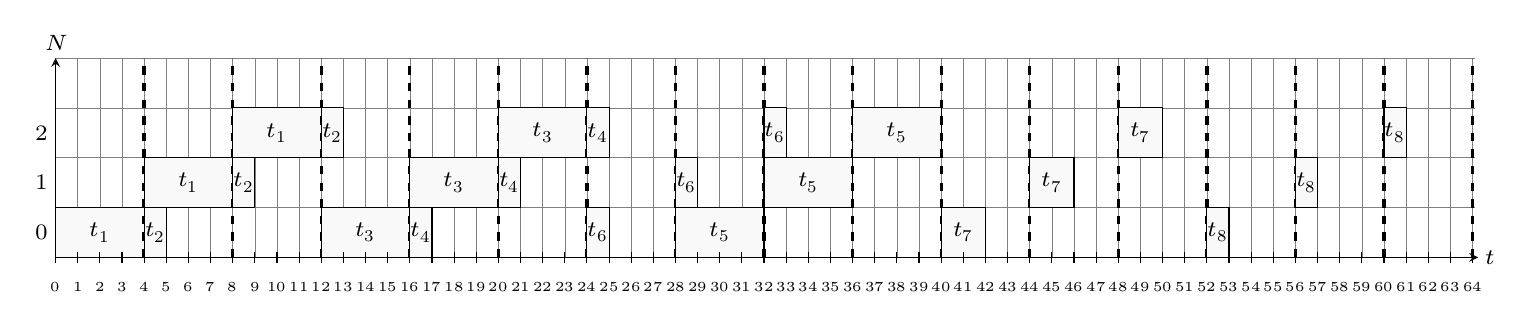
\begin{tikzpicture}[x = 0.8em, y = 1.8em]
								\footnotesize
								\draw[help lines, step=1] (0.0, 0.0) grid (64.1, 4.0);

								% Coordinate lines
								\begin{scope}[>=stealth]
									\draw[->] (0, 0) -- (64.25, 0) node[right] {$t$};
									\draw[->] (0, 0) -- (0, 4)   node[above] {$N$};
								\end{scope}

								\begin{scope}
									% step 01
									%
									\draw [fill = black!2.5]  (00,00) rectangle node {$t_1$} (04,01);
									\draw [dashed, very thick] (04,00) -- (04,04);
									% step 02
									%
									\draw [fill = black!2.5]  (04,00) rectangle node {$t_2$} (05,01);
									\draw [fill = black!2.5]  (04,01) rectangle node {$t_1$} (08,02);
									\draw [dashed, very thick] (08,00) -- (08,04);
									% step 03
									%
									\draw [fill = black!2.5]  (08,01) rectangle node {$t_2$} (09,02);
									\draw [fill = black!2.5]  (08,02) rectangle node {$t_1$} (12,03);
									\draw [dashed, very thick] (12,00) -- (12,04);
									% step 04
									%
									\draw [fill = black!2.5]  (12,00) rectangle node {$t_3$} (16,01);
									\draw [fill = black!2.5]  (12,02) rectangle node {$t_2$} (13,03);
									\draw [dashed, very thick] (16,00) -- (16,04);
									% step 05
									%
									\draw [fill = black!2.5]  (16,00) rectangle node {$t_4$} (17,01);
									\draw [fill = black!2.5]  (16,01) rectangle node {$t_3$} (20,02);
									\draw [dashed, very thick] (20,00) -- (20,04);
									% step 06
									%
									\draw [fill = black!2.5]  (20,01) rectangle node {$t_4$} (21,02);
									\draw [fill = black!2.5]  (20,02) rectangle node {$t_3$} (24,03);
									\draw [dashed, very thick] (24,00) -- (24,04);
									% step 07
									%
									\draw [fill = black!2.5]  (24,00) rectangle node {$t_6$} (25,01);
									\draw [fill = black!2.5]  (24,02) rectangle node {$t_4$} (25,03);
									\draw [dashed, very thick] (28,00) -- (28,04);
									% step 08
									%
									\draw [fill = black!2.5]  (28,00) rectangle node {$t_5$} (32,01);
									\draw [fill = black!2.5]  (28,01) rectangle node {$t_6$} (29,02);
									\draw [dashed, very thick] (32,00) -- (32,04);
									% step 09
									%
									\draw [fill = black!2.5]  (32,01) rectangle node {$t_5$} (36,02);
									\draw [fill = black!2.5]  (32,02) rectangle node {$t_6$} (33,03);
									\draw [dashed, very thick] (36,00) -- (36,04);
									% step 09
									%
									\draw [fill = black!2.5]  (36,02) rectangle node {$t_5$} (40,03);
									\draw [dashed, very thick] (40,00) -- (40,04);
									% step 09
									%
									\draw [fill = black!2.5]  (40,00) rectangle node {$t_7$} (42,01);
									\draw [dashed, very thick] (44,00) -- (44,04);
									% step 10
									%
									\draw [fill = black!2.5]  (44,01) rectangle node {$t_7$} (46,02);
									\draw [dashed, very thick] (48,00) -- (48,04);
									% step 11
									%
									\draw [fill = black!2.5]  (48,02) rectangle node {$t_7$} (50,03);
									\draw [dashed, very thick] (52,00) -- (52,04);
									% step 12
									%
									\draw [fill = black!2.5]  (52,00) rectangle node {$t_8$} (53,01);
									\draw [dashed, very thick] (56,00) -- (56,04);
									% step 13
									%
									\draw [fill = black!2.5]  (56,01) rectangle node {$t_8$} (57,02);
									\draw [dashed, very thick] (60,00) -- (60,04);
									% step 14
									%
									\draw [fill = black!2.5]  (60,02) rectangle node {$t_8$} (61,03);
									\draw [dashed, very thick] (64,00) -- (64,04);
								\end{scope}

								\newcommand*{\TickSize}{0.25em}
								% x ticks
								\begin{scope}
									\foreach \x in {0,...,64} {%
											\draw ($(\x,0) + (0,-\TickSize)$) -- ($(\x,0) + (0,\TickSize)$)
													node [anchor = north, below = 1em, font={\tiny}] {$\x$};
									}
								\end{scope}
								% y ticks
								% \begin{scope}
								% 	\foreach \y in {0,...,3} {%
								% 			\draw ($(0,\y) + (-\TickSize,0)$) -- ($(0,\y) + (\TickSize,0)$)
								% 					node [anchor = east, left = 1em] {CPU $\y$};
								% 	}
								% \end{scope}

								\begin{scope}
									\foreach \y in {0,...,2} {%
										\node[anchor = east] at (0, \y + 0.5) {$\y$};
									}
								\end{scope}
							\end{tikzpicture}
							\caption{Часова діаграма роботи конвеєра типу~K1 при~кількості шарів~$N = 3$}
							\label{fig:time-diag-pipeline-usage-k1}
						\end{figure}
					\end{landscape}
				}

				Як~видно на~осі~$Ot$, найдовший відрізок займає~64 одиниці, тобто виконання обчислення займає~$T_{K1} = 64 t_{+}$.

				Обчисливши тривалість виконання обчислення на~обчислювальній системі типу K1 з~кількістю шарів~$N = 3$, обчислюємо її~критерії ефективності: коефіцієнт прискорення~$K_{\text{П}}$ і~коефіцієнт завантаження~$K_{\text{З}}$. Вони обчислюються так:
				\begin{IEEEeqnarray*}{rCl}
					K_{\text{П}} = \frac{T_0}{T_{K1}} = \frac{48 t_{+}}{64 t_{+}} = \num{0.750}, \quad
					K_{\text{З}} = \frac{T_0}{N \cdot T_{K1}} = \frac{48 t_{+}}{3 \cdot 64 t_{+}} = \num{0.250}.
				\end{IEEEeqnarray*}
				Отже, отримали характеристики ефективності конвеєрної системи типу~K1.

	\section{Висновок}
		Виконуючи дану лабораторну роботу, ми~проаналізували функціонування та~ефективність конвеєрів різних типів, а також визначили характеристики їх ефективності~(табл.~\ref{tab:efficiency-comparison}).
		\begin{table}[!htbp]
			\centering
			\caption{Характеристики ефективності розглянутих типів конвеєрів}
			\label{tab:efficiency-comparison}
			\begin{tabular}{
				v{3\gridunitwidth - 2\tabcolsep}
				n{2\gridunitwidth - 2\tabcolsep}
				n{2\gridunitwidth - 2\tabcolsep}
			}
				\toprule
					Тип конвеєра & $K_{\text{П}}$ & $K_{\text{З}}$\\
				\midrule
					К2.1 & \num{1.231} & \num{0.410}\\
					К2.2 & \num{1.200} & \num{0.400}\\
					К1   & \num{0.750} & \num{0.250}\\
				\bottomrule
			\end{tabular}
		\end{table}

		Зі~значень визначених характеристик можна зробити такі висновки:
		\begin{enumerate}
			\item Використання конвеєру типу~K2.1 дозволяє розв'язати задачу за~мінімальний час та~з~максимальним використанням обладнання.
			\item Конвеєр типу~K2.2 лише назначно поступається конвеєру типу~K2.1 у~швидкості розв'язання задачі та~степені використання обладнання.
			\item Конвеєр типу~K1 сповільнює обчислення виразу.
		\end{enumerate}
		Тому варто відмовитись від конвеєра типу~K1, адже він сповільнює виконання задачі і~водночас потребує зусиль на~реалізацію. Слід віддати перевагу конвеєру типу~K2.2, оскільки він є~найдійнішим, дешевшим та~легшим у~реалізації, ніж конвеєр типу~K2.1.

\end{document}

